\subsection{Conceptos claves}
\begin{itemize}
    \item \textbf{Microrred:} cluster de generación distribuida , fuentes locales y cargas que permiten conectarse mediante una red eléctrica en la que se gestiona integralmente la generación, el almacenamiento de energía y las necesidades de las cargas de los usos finales \cite{microgrid}.
    \item \textbf{Sistemas de Almacenamiento de Energía por Baterías (BESS)}: sistema recargable de baterías capaz de almacenar energía de diferentes fuentes y descargarse cuando se necesite. BESS consta de una o más baterías y se puede utilizar para equilibrar la red eléctrica, proporcionar energía de respaldo y mejorar la estabilidad de la red \cite{siemens}.
    \item  \textbf{Estado de Carga (SoC):} medida relativa de la cantidad de energía almacenada en una batería, definida como la relación entre la cantidad de carga extraíble de la celda en un momento específico del tiempo y la capacidad total.
    \item \textbf{Inversor DC-AC:} su función es transformar una tensión de entrada continua a una tensión de salida alterna con una magnitud y frecuencia deseada \cite{rashid-inversor}. El proceso de conmutación se realiza generalmente con transistores MOSFET e IGBT mediante señales PWM con el objetivo de obtener a la salida una señal sinusoidal.
    \item \textbf{Densidad de energía:} cantidad de energía que se puede almacenar en un solo sistema por unidad de volumen o por unidad de peso \cite{densidad}.
\end{itemize}

\newpage
La producción de energía eléctrica es una necesidad del mundo moderno del cual el ser humano no puede prescindir. Por lo tanto, los sistemas de energía eléctrica deben tener la capacidad de suministrar energía suficiente para la cantidad demandada teniendo en cuenta la calidad del servicio, las condiciones ambientales y los costos. Debido a que existe variabilidad en la producción de energías tanto  convencionales y no convencionales, se requiere almacenar energía para maximizar su aprovechamiento. 


\subsection{Tipos de almacenamiento en la red}
En la actualidad existen diferentes tipos de tecnologías para almacenamiento de energía (ESS) dependiendo de su uso. Los dispositivos de almacenamiento se pueden clasificar en mecánicos, electroquímicos, químicos, eléctricos y térmicos \cite{Handbook}. En la Figura 8, se pueden visualizar los tipos de ESS.
\begin{figure}[h!]
    \begin{center}
    \centering
    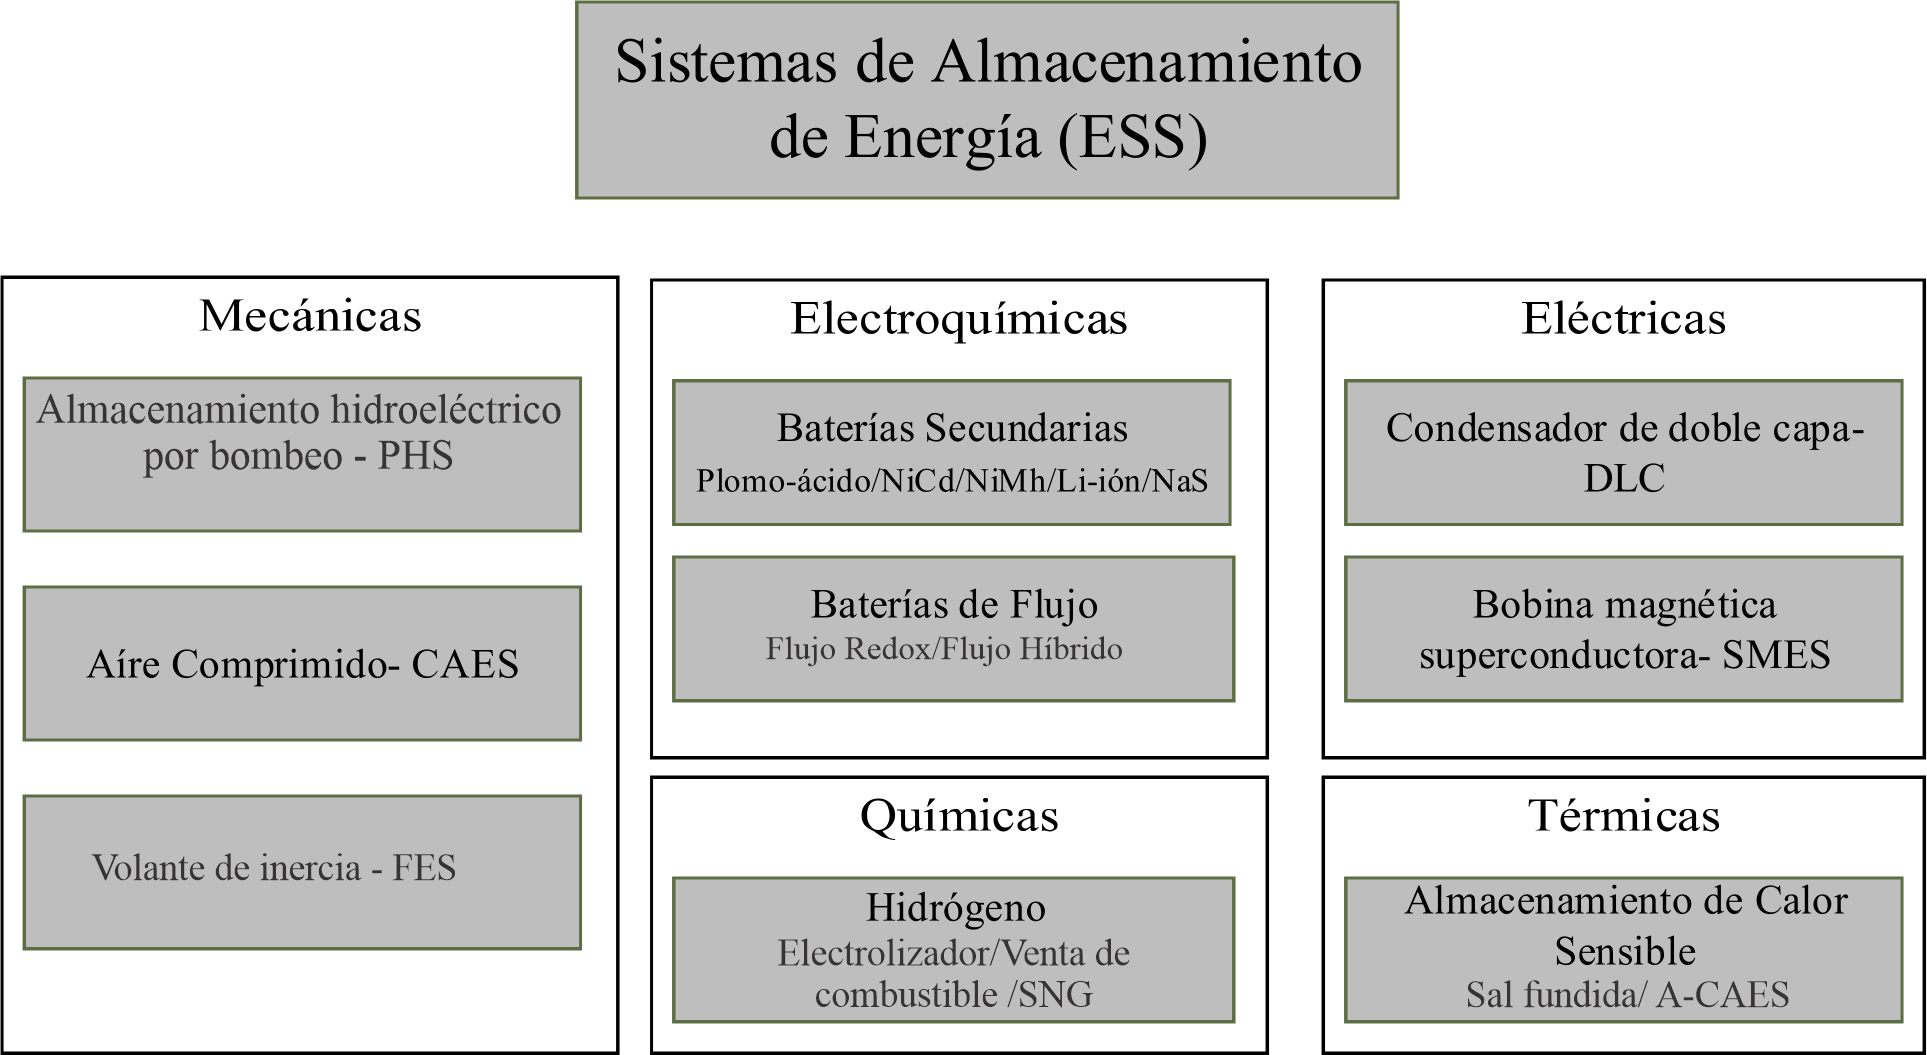
\includegraphics[scale=0.7]{Imágenes/marcoconceptual/Tipos de energias.png}
	\caption{ Clasificación de  los sistemas de almacenamiento de energía (ESS)\cite{bess_distritall}.}
    \end{center}
\end{figure}
\newpage
Los dispositivos de almacenamiento tienen dos fines principales, el suministro de energía ininterrumpida (UPS) o transmisión y soporte del sistema de distribución \cite{Handbook}. En la Tabla 1, se visualiza una comparación más detallada de diferentes tecnologías ESS, clasificándolas por su duración del almacenamiento, número de ciclos o vida útil, autodescarga, densidad de  potencia y tiempo de respuesta.
\begin{table}[htbp]
  \centering
  \caption{Características técnicas de los ESS }
  \resizebox{17cm}{!} {
    \begin{tabular}{|p{13.855em}|c|c|c|c|c|}
    %\toprule
    \rowcolor[rgb]{ .051,  .051,  .051} \multicolumn{1}{|c|}{\textcolor[rgb]{ 1,  1,  1}{\textbf{PARÁMETROS }}} & \multicolumn{1}{p{10.145em}|}{\textcolor[rgb]{ 1,  1,  1}{\textbf{Densidad de potencia (Wkg/kWm)}}} & \multicolumn{1}{p{8.57em}|}{\textcolor[rgb]{ 1,  1,  1}{\textbf{Tiempo de vida (años-ciclos) }}} & \multicolumn{1}{p{8.285em}|}{\textcolor[rgb]{ 1,  1,  1}{\textbf{Tiempo de descarga tipico}}} & \textcolor[rgb]{ 1,  1,  1}{\textbf{Tiempo de recarga }} & \multicolumn{1}{p{8.855em}|}{\textcolor[rgb]{ 1,  1,  1}{\textbf{Auto descarga (\%\textbackslash{}día)}}} \\
    %\midrule
    \rowcolor[rgb]{ .051,  .051,  .051} \multicolumn{1}{|c|}{\textcolor[rgb]{ 1,  1,  1}{\textbf{TECNOLOGÍAS}}} & \textcolor[rgb]{ 1,  1,  1}{} & \textcolor[rgb]{ 1,  1,  1}{} & \textcolor[rgb]{ 1,  1,  1}{} & \textcolor[rgb]{ 1,  1,  1}{} & \textcolor[rgb]{ 1,  1,  1}{} \\
    %\midrule
    \multicolumn{1}{|c|}{Volantes de Inercia} & 400-1600/5000 & >20 (10$^7$) & 15 s-15 min & <15 min & 20-100 \\
    \hline
    \rowcolor{gris} \multicolumn{1}{|c|}{Hidroeléctrica bombeada} & NA/0.1-0.2 & 50-100 (>500) & h-days & 1 min-h & 0 \\
    \hline
    \multicolumn{1}{|c|}{Aire Comprimido} & NA/0.2-0.6 & 25-40  & h-days & min-h & 0 \\
    \hline
    \rowcolor{gris} Supercapacitores/Capacitores de doble capa & 0.1-10/40000-120000 & >20 (5x10$^5$) & ms-1 h & s-min & 2-.40 \\
    \hline
    \multicolumn{1}{|c|}{Batería Ión de litio} & 230-340/1300-10000 & 8-15 (500-6000) & min-h & min-h & 0.1-0.3 \\
    \hline
    \rowcolor{gris} \multicolumn{1}{|c|}{Batería de Cadmio de Níquel} & 150-300/75-700 & 15-20 (2500) & s-h   & 1 h   & 0.2-0.6 \\
    \hline
    \multicolumn{1}{|c|}{Batería Sulfuro de Sodio} & 90-230/120-160 & 12-20 (>2000) & s-h   & 9 h   & 20 \\
    \hline
    \rowcolor{gris} Supercapacitores/Capacitores de doble capa & 0.1-10/40000-120000 & >20 (5x10$^5$) & ms-1 h & s-min & 2-.40 \\
    \hline
    \multicolumn{1}{|c|}{Batería de Ácido de Plomo} & 75-300/90-700 & 3-15 (2000) & min-h & 8-16 h & 0.1-0.3 \\
    \hline
    \rowcolor {gris} \multicolumn{1}{|c|}{Batería de Bromuro de Zinc} & 50-150/1-25 & 5-10 (300-1500) & s-10 h & 4 h   & 0-1 \\
    \hline
    Batería de Reducción-Oxidación de Vanadio & NA/0.5-2 & 10-20 (13x10$^3$) & s-10 h & min   & 0-10 \\
    \bottomrule
    \end{tabular}%
    }
  \label{tab:addlabel}%
\end{table}%
\newline
Los sistemas BESS se consideran tecnologías de tiempo de descarga medio (duración entre varios minutos hasta algunas horas) con tecnologías electroquímicas \cite{bess_distritall}. Las tecnologías de baterías para dispositivos de almacenamiento de energía se pueden diferenciar en función de la densidad de energía, tiempo de carga y descarga, esperanza de vida y el impacto ambiental \cite{Handbook}.
\newpage
\begin{table}[htbp]

  \centering
  \caption{Comparación técnicas de los BESS}
  \resizebox{16cm}{!} {
    \begin{tabular}{|p{10em}|c|c|c|c|c|p{11em}|}
    %\toprule
    \rowcolor[rgb]{ .051,  .051,  .051} \multicolumn{1}{|c|}{\textcolor[rgb]{ 1,  1,  1}{\textbf{PARÁMETROS }}} & \multicolumn{1}{p{10em}|}{\textcolor[rgb]{ 1,  1,  1}{\textbf{Potencia AC nominal}}} & \multicolumn{1}{p{10em}|}{\textcolor[rgb]{ 1,  1,  1}{\textbf{Autodescarga}}} & \multicolumn{1}{p{10em}|}{\textcolor[rgb]{ 1,  1,  1}{\textbf{Profundidad de descarga \%}}} & \multicolumn{1}{p{10em}|}{\textcolor[rgb]{ 1,  1,  1}{\textbf{Eficiencia Roundtrip \newline{}\%}}} & \multicolumn{1}{p{10em}|}{\textcolor[rgb]{ 1,  1,  1}{\textbf{Temperatura óptima de diseño}}} & \textcolor[rgb]{ 1,  1,  1}{\textbf{Aplicación}} \\
    %\midrule
    \rowcolor[rgb]{ .051,  .051,  .051} \multicolumn{1}{|c|}{\textcolor[rgb]{ 1,  1,  1}{\textbf{BATERÍAS}}} & \textcolor[rgb]{ 1,  1,  1}{} & \textcolor[rgb]{ 1,  1,  1}{} & \textcolor[rgb]{ 1,  1,  1}{} & \textcolor[rgb]{ 1,  1,  1}{} & \textcolor[rgb]{ 1,  1,  1}{} & \multicolumn{1}{r|}{\textcolor[rgb]{ 1,  1,  1}{}} \\
    %\midrule
    \multicolumn{1}{|c|}{Ión de Litio} & \multicolumn{1}{|c|}{200-500 kW} & 1-2\% mensual  & 100   & 85-95 & 15°C  & Cámaras,  computadores portátiles y dispositivos móviles  \\
    \hline
    \rowcolor{gris} \multicolumn{1}{|c|}{Sulfuro de Sodio} & 50-400 kW & 0.01\%  mensual  & 100   & 89-92 & 300°C–350°C &  Redes de almacenamiento de energía fijas a gran escala \\
    \hline
    \multicolumn{1}{|c|}{Flujo redox} & 50-330 kW & Baja  & 100   & 85-90 & 5°C–35°C &  Aplicaciones \newline{}estacionarias  \\
    \hline
    \rowcolor{gris} \multicolumn{1}{|c|}{Plomo Ácido} & 250-500 kW & 0.1\% mensual & 50    & 80-85 & 45°C  & Sistema de alimentación ininterrumpida o en sistemas   de energía renovable \\
    \hline
    \multicolumn{1}{|c|}{ Níquel-Cadmio} & 125-600 kW & 15-20\% mensual & 50    & 70-90 & 5°C-25°C & Computadores portátiles, taladros, cámaras de video  y otros dispositivos que requieren una descarga  uniforme. \\
    \hline
    \rowcolor{gris} Níquel-Metalhidruro & 500-2000 W & 30\% mensual & 100   & 66    & -30°C a 70°C &  Vehículos, robótica y en electrónica de consumo.    \\
    \bottomrule
    \end{tabular}%
    }
  \label{tab:addlabel}%
  
\end{table}%







Existen diferentes tipos de tecnologías de baterías en el mercado, en la Tabla 2 se realiza una comparación de características técnicas de diferentes baterías en el mercado, especificando los siguientes parámetros:
\begin{itemize}
    \item Potencia AC nominal: ``potencia máxima empleada por una máquina en uso normal" \cite{proyecto_mg}.
    \item Profundidad de descarga: ``la cantidad de energía que se ha extraído de la batería, expresada en porcentaje" \cite{profundidad_descarga}.
    \item Eficencia Roadtrip: ``tiempo de ida y vuelta (RTT) es la duración en milisegundos que tarda una solicitud de red en ir de un punto de partida a un destino y volver al punto de partida" \cite{tiempo_ida_vuelta}.
\end{itemize}
